\documentclass{article}
\usepackage[utf8]{inputenc}
\usepackage{amsmath,amsfonts,amssymb,amsthm}
%\usepackage{mathtools}
\usepackage{graphicx}
\usepackage{setspace}
% \usepackage[a4paper, total={6in, 8in}]{geometry}
\usepackage[top=2.5cm, left=2.0cm, right=2.0cm, bottom=3.0cm]{geometry}

\title{%
    Exercise 2 \\
    \large Foundations of Data Science 
}
\author{Wenjie Tu}
\date{Fall 2020}

\setlength{\parindent}{0pt}
%\setlength{\parskip}{1em}
%\onehalfspacing
\begin{document}

\maketitle

\textbf{1. Logical Gates Using Perceptron}

\[y=
    \begin{cases}
    1, & \textrm{if } w_0+\sum_{i=1}^{D}w_ix_i\geq 0 \\
    -1, & \textrm{otherwise}
    \end{cases}
\]

\textbf{1. a}

The truth table for \textbf{AND} gate:

\begin{table}[h]
    \centering
    \begin{tabular}{c|c|c}
    \hline
    $x_1$ & $x_2$ & $x_1$ AND $x_2$  \\
    \hline 
    $ 0 $ & $ 0 $ & $ -1 $ \\
    \hline
    $ 0 $ & $ 1 $ & $ -1 $ \\
    \hline
    $ 1 $ & $ 0 $ & $ -1 $ \\
    \hline
    $ 1 $ & $ 1 $ & $  1 $ \\
    \hline
    \end{tabular}
    % \caption{The truth table for \textbf{AND} gate}
    % \label{tab:my_label}
\end{table}

A perceptron that simulates an \textbf{AND} gate:

\[
y=
\begin{cases}
    1, & \textrm{if } -2+x_1+x_2\geq 0 \\
    -1, & \textrm{otherwise}
\end{cases}
\]

The truth table for \textbf{OR} gate:

\begin{table}[h]
    \centering
    \begin{tabular}{c|c|c}
    \hline
    $x_1$ & $x_2$ & $x_1$ OR $x_2$  \\
    \hline 
    $ 0 $ & $ 0 $ & $ -1 $ \\
    \hline
    $ 0 $ & $ 1 $ & $  1 $ \\
    \hline
    $ 1 $ & $ 0 $ & $  1 $ \\
    \hline
    $ 1 $ & $ 1 $ & $  1 $ \\
    \hline
    \end{tabular}
    % \caption{Caption}
    % \label{tab:my_label}
\end{table}

A perceptron that simulates an \textbf{OR} gate:

\[
y=
\begin{cases}
    1, & \textrm{if } -1+x_1+x_2\geq 0 \\
    -1, & \textrm{otherwise}
\end{cases}
\]

The truth table for \textbf{NOT} gate:

\begin{table}[h]
    \centering
    \begin{tabular}{c|c}
    \hline
    $x_1$ & NOT $x_1$  \\
    \hline 
    $ 0 $ & $ 1 $ \\
    \hline
    $ 1 $ & $ 0 $ \\
    \hline
    \end{tabular}
    % \caption{Caption}
    % \label{tab:my_label}
\end{table}


A perceptron that simulates an \textbf{NOT} gate:

\[
y=
\begin{cases}
    1, & \textrm{if } -x_1\geq 0 \\
    -1, & \textrm{otherwise}
\end{cases}
\]

\textbf{1. b}

The truth table for \textbf{XOR} gate:

\begin{table}[h]
    \centering
    \begin{tabular}{c|c|c}
    \hline
    $x_1$ & $x_2$ & $x_1$ XOR $x_2$  \\
    \hline 
    $ 0 $ & $ 0 $ & $ -1 $ \\
    \hline
    $ 0 $ & $ 1 $ & $  1 $ \\
    \hline
    $ 1 $ & $ 0 $ & $  1 $ \\
    \hline
    $ 1 $ & $ 1 $ & $ -1 $ \\
    \hline
    \end{tabular}
    % \caption{Caption}
    % \label{tab:my_label}
\end{table}

Since the XOR function is not linearly separable, it is impossible for a single perceptron to simulate such a gate.

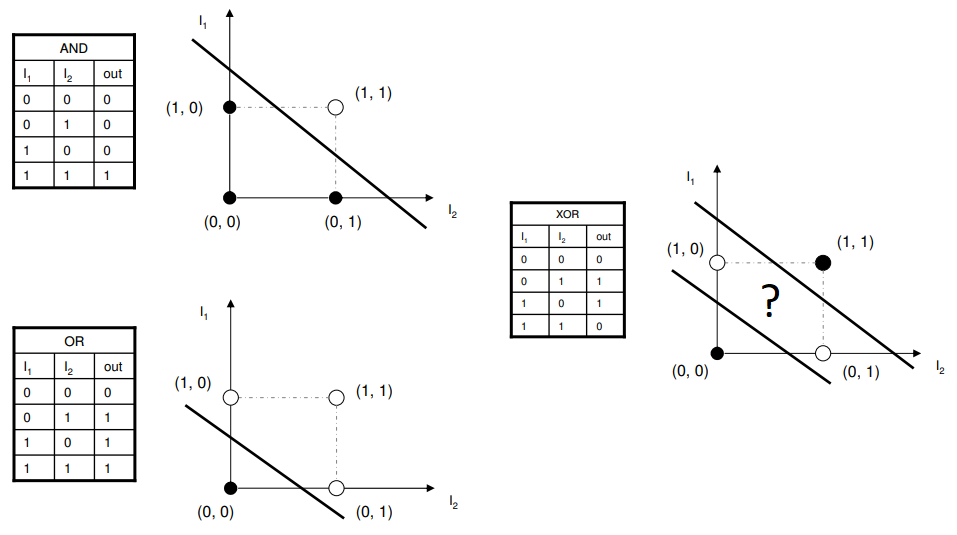
\includegraphics[scale=0.5]{logic_gate.png}

\textbf{1. c}

The truth table for \textbf{SAME} gate:

\begin{table}[h]
    \centering
    \begin{tabular}{c|c|c}
    \hline
    $x_1$ & $x_2$ & $x_1$ SAME $x_2$  \\
    \hline 
    $ 0 $ & $ 0 $ & $  1 $ \\
    \hline
    $ 0 $ & $ 1 $ & $  0 $ \\
    \hline
    $ 1 $ & $ 0 $ & $  0 $ \\
    \hline
    $ 1 $ & $ 1 $ & $  1 $ \\
    \hline
    \end{tabular}
    % \caption{Caption}
    % \label{tab:my_label}
\end{table}

\textbf{1. d}

\[
\tanh(z)=\frac{e^z-e^{-z}}{e^z+e^{-z}}
\]

\[
y=
\begin{cases}
1, & \tanh\left(w_0+\sum_{i=1}^{D}w_ix_i \right)>0.99 \\
-1, & \tanh\left(w_0+\sum_{i=1}^{D}w_ix_i \right)<-0.99
\end{cases}
\]

\vspace{5mm}

\textbf{2. Nearest Neighbor Classification}

\textbf{2. a}

What advantage does the $k$-NN approach offer over a linear classifier like the perceptron?

\begin{itemize}
    \item A $k$-NN classifier is non-linear since its decision boundary on the feature space is a non-linear function.
    \item A perceptron is linear since its decision boundary on the feature space is a linear function.
\end{itemize}

If a classification problem is non-linear separable and the decision boundary cannot be approximated well with a linear hyperplane, non-linear classifiers (e.g., $k$-NN) are more accurate than linear classifiers (e.g., perceptron). 

\vspace{5mm}


\textbf{3. Linear Regression and Basis Expansion}

\textbf{3. a}

\[
y_i=w_0+w_1x_i,\quad\text{for $i\in\{1,\cdots,6\}$}
\]

\[
\mathbf{X}=
\begin{bmatrix}
1 & 2 \\ 1 & 3 \\ 1 & 4 \\ 1 & 5 \\ 1 & 6 \\ 1 & 7
\end{bmatrix},
\quad
\mathbf{y}=
\begin{bmatrix}
5 \\ 6 \\ 5 \\ 9 \\ 7 \\ 10
\end{bmatrix}
\]

The least squares estimator:

\[
\mathbf{w}=(\mathbf{X}^{\intercal}\mathbf{X})^{-1}\mathbf{X}^{\intercal}\mathbf{y}
\approx
\begin{bmatrix}
2.89 \\ 0.91
\end{bmatrix}=
\begin{bmatrix}
w_0 \\w_1
\end{bmatrix}
\]

\textbf{3. b}

\[
y_i=w_0+w_1x_i+w_2x_i^2,\quad\text{for $i\in\{1,\cdots,6\}$}
\]

\[
\mathbf{X}=
\begin{bmatrix}
1 & 2 & 2^2 \\ 1 & 3 & 3^2 \\ 1 & 4 & 4^2 \\ 1 & 5 & 5^2 \\ 1 & 6 & 6^2 \\ 1 & 7 & 7^2
\end{bmatrix},
\quad
\mathbf{y}=
\begin{bmatrix}
5 \\ 6 \\ 5 \\ 9 \\ 7 \\ 10
\end{bmatrix}
\]

\[
\mathbf{w}=(\mathbf{X}^{\intercal}\mathbf{X})^{-1}\mathbf{X}^{\intercal}\mathbf{y}
\approx
\begin{bmatrix}
4.74 \\ -0.05 \\ 0.11
\end{bmatrix}=
\begin{bmatrix}
w_0 \\w_1 \\ w_2
\end{bmatrix}
\]

\textbf{3. c}

\[
\textrm{MSE}=\frac{1}{2N}\sum_{i=1}^{N}(y-\hat{y})^2
\]

\begin{itemize}
    \item In 3. a with a linear model, $\textrm{MSE}=0.62$
    \item In 3. b with a nonlinear model, $\textrm{MSE}=0.58$
\end{itemize}

\textbf{3. d}

Overfitting.

\vspace{5mm}

\textbf{4. Predicting Commute Time}

\textbf{4. a}

\[
y=w_0+w_1x_{dist}+w_2x_{weekd}+\varepsilon
\]

\begin{itemize}
    \item $w_0$: bias term.
    \item $x_{dist}$: real feature for distance.
    \item $weekd$: boolean featire for weekday or weekend.
    \item $\varepsilon$: noise term.
\end{itemize}

\underline{First trial:}

\begin{itemize}
    \item Introduce 7 boolean features for Monday, Tuesday, ..., Sunday.
    \item For each data point, exactly one of these features is 1.
\end{itemize}

Implications:

\begin{itemize}
    \item Columns of data matrix are linearly dependent.
    \item $\mathbf{X}^{\intercal}\mathbf{X}$ is not invertible.
\end{itemize}

\underline{Better approach:}

\begin{itemize}
    \item Introduce 7 boolean features for Monday, Tuesday, ..., Saturday.
    \item For each data point, at most one of these features is 1.
    \item If all these features are 0, it means Sunday.
\end{itemize}

Model:

\[
y=w_0+w_1x_{dist}+w_2x_{mon}+\cdots+w_7x_{sat}+\varepsilon
\]

\textbf{4. b}

Introduce a Boolean feature $x_{vehicle}$:

\[
x_{vehicle}=
\begin{cases}
1, & \text{car is used} \\
0, & \text{bus is used}
\end{cases}
\]

Model:

\[
y=w_0+w_1x_{dist}+w_2x_{mon}+\cdots+w_7x_{sat}+w_8x_{vehicle}+\varepsilon
\]

\underline{How to make suggestions?}

\begin{itemize}
    \item Train the model.
    \item For given $x_{dist}, x_{mon}, \cdots, x_{sat}$, predict with $x_{vehicle}=1$ and with $x_{vehicle}=0$.
    \item Suggest car if prediction with $x_{vehicle}=1$ is better than prediction with $x_{vehicle}=0$.
\end{itemize}

\textbf{4. c}

Use a model for each time frame.

\underline{How to make suggestions?}

\begin{itemize}
    \item Train the model.
    \item For given $x_{dist},x_{mon},\cdots,x_{sat}$, use each model to predict the commute time within a specific time frame.
    \item Suggest time frame $i$ if $y_{ti}$ predicts the lowest commute time.
\end{itemize}

\vspace{4mm}

\textbf{5. Predicting Jogging Time}

\textbf{5. a}

\[
x_{t+1}=w_0+w_1x_t+w_2x_{t-1}+\varepsilon
\]

\textbf{5. b}

\[
\Delta_{t+1}=w_0+w_1x_t+w_2x_{t-1}+\varepsilon
\]

Note that $\Delta_{t+1}:=x_{t+1}-x_t$.

\textbf{5. c}

\[
\Delta_{t+1}=w_0+w_1\Delta_{t}+\varepsilon
\]

\textbf{5. d}

\[
\Delta_{t+1}=w_0+w_1x_t+w_2\Delta_{t}+\varepsilon
\]

\vspace{4mm}

\textbf{6. The Huber Loss in a Linear Regression Setting}

Huber loss function:

\[
h_{\lambda,\mu}(z)=
\begin{cases}
\lambda\left(|z|-\frac{\lambda}{4\mu} \right), & \textrm{if $|z|\geq\frac{\lambda}{2\mu}$} \\
\mu z^2, & \textrm{otherwise}
\end{cases}
\]

Absolute loss function:

\[
f(z)=|z|
\]

Square loss function:

\[
g(z)=z^2
\]

\textbf{6. a}



\end{document}
